\chapter{Calcolabilita' relativa e gerarchia polinomiale}

Uno dei problemi della macchina di Turing e' che non e' un formalismo composizionale. E' difficile
comporre assieme due Macchine di Turing, e' una cosa che dobbiamo fare al di fuori del linguaggio.
Il formalismo non permette di farlo in modo interno.

L'idea di fondo del concetto di oracolo e' quella di permettere ad una MdT $M$ di fare chiamate
esterne ad un agente che chiamiamo oracolo. Un oracolo per un linguaggio $\Lang$ e', idealmente, un
qualcosa che, data una stringa $x$ in input, risponde in tempo costante e in modo corretto alla
domanda $x \in \Lang$. Non e' necessario che il linguaggio per cui vogliamo un oracolo sia
decidibile.

Il problema di studio diventa, a questo punto, supponendo di avere questo oracolo, cosa riusciamo a
calcolare e con quale complessita'? Tanto piu' il linguaggio gestito dall'oracolo e' potente tanto
piu' aumenta il nostro potere espressivo. La possibilita' di interagire con un oracolo potente
aumenta il nostro potere computazionale.

L'oracolo e' stato introdotto in teoria della calcolabilita', dove ci si chiede cosa riusciamo a
calcolare, ad esempio, con un oracolo per il problema della terminazione. Abbiamo un aumento nel
potere computazionale, ma non cosi' esteso come si potrebbe pensare. In effetti questo e'
intuitivamente comprensibile, dato che il problema della terminazione si posiziona molto in basso
nella gerarchia aritmetica.

Dal punto di vista della teoria della complessita' siamo interessati a sapere quale sia la
complessita' richiesta per interrogare l'oracolo. Noi supponiamo che l'interrogazione all'oracolo
costi $O(1)$. Il costo della prepararazione dell'interrogazione e' a carico del chiamante. In questo
modo ci possiamo concentrare direttamente sulla complessita' della macchina chiamante,
indipendentemente dalle chiamate all'oracolo. Questo corrisponde, nell'analisi di un algoritmo,
all'ignorare certe chiamate di funzione nell'analisi di costo, il che e' lecito quando siamo
interessati a parti dell'algoritmo a prescindere dalla complessita' delle subroutine chiamate.

%Slide 142
\section{Macchine di Turing con Oracolo}

La formalizzazione della MdT con oracolo e' semplice. Rispetto alla MdT tradizionale abbiamo 3 stati
nuovi e un nuovo nastro per fare l'interrogazione all'oracolo. Per interrogare l'oracolo scriviamo
su questo nastro e otteniamo, in $O(1)$, la risposta. Abbiamo uno stato di interrogazione, $q?$, uno
stato $q+$, per una risposta positiva dell'oracolo, e $q-$ per una risposta negativa.

Il nastro di interrogazione e' un nastro come gli altri, e la MdT puo' usarlo come vuole. La
funzione di transizione $\delta$ non e' definita sullo stato di interrogazione $q?$. Quando la MdT
entra nello stato di interrogazione lo stato successivo non e' deciso dalla sua $\delta$, ma
dall'oracolo. Se al momento del passaggio allo stato $q?$ sul nastro dell'oracolo alla sinistra
della testina la MdT ha scritto la stringa $x$, l'oracolo $O$ per il linguaggio $O$ (denotiamo
oracolo e linguaggio deciso dall'oracolo con lo stesso simbolo) pone la MdT nello stato $q+$ se $x \in
O$, e, viceversa, pone la MdT nello stato $q-$ se $x \notin O$. Il contenuto del nastro di
interrogazione e' cancellato automaticamente non appena la MdT rientra nello stato $q+$ o $q-$.
Denotiamo la MdT $M$ che utilizza un oracolo $O$ con $M^{O}$.

Fissate queste condizioni possiamo scrivere dei programmi per la MdT $M$ con oracolo $O$. Non
cambiano le nozioni di tempo e spazio consumati da $M^{O}$. Possiamo avere macchine deterministiche
o non deterministiche con oracolo.

%Slide 145
\section{Classi di complessita' con oracolo}

Supponiamo di avere un determinato oracolo per un dato linguaggio $O$, e indichiamolo con $O$.  In
generale usiamo un apice con $O$ per indicare la computazione relativizzata che usa chiamate
all'oracolo $O$.  Si definisce una classe $\CClass^{O}$ in modo analogo alla definizione di
$\CClass$, ma aggiungendo $\CClass$ quei linguaggi che possono essere riconosciuti con le stesse
risorse della classe utilizzando interrogazioni all'oracolo $O$.

Ad esempio, $\PClass^{\SAT}$ e' la clase dei linguaggi riconoscibili in tempo polinomiale
permettendo interrogazioni ad un oracolo per $\SAT$.

Definiamo classi $\CClass$ relativizzate rispetto a classi $\CClass'$ come l'unione, per ogni
linguaggio $O$ in $\CClass'$, delle classi $\CClass^{O}$:
\begin{equation*}
    \CClass^{\CClass'} = \bigcup_{O \in \CClass'}\CClass^{O}
\end{equation*}
Nota: la $O$ nel pedice dell'unione indica un linguaggio, mentre la $O$ in apice a $\CClass$ indica
un oracolo. Le classi di complessita', anche relativizzate, rimangono classi di linguaggi.

Dire che un linguaggio $\Lang$ appartiene a $\CClass^{\CClass'}$ non siginifica dire che esiste una
MdT $M$ che riconosce $\Lang$ facendo chiamate a tante oracoli. Per definizione una MdT lavora con
un solo oracolo. Quindi, $\Lang \in \CClass^{\CClass'} \iff \exists O \in \CClass'. \Lang \in
\CClass^{O}$. Se volessimo lavorare con piu' oracoli avremmo bisogno, con la definizione data, di un
oracolo unico che ``aggreghi'' tutti gli oracoli che ci servono.

Nonostante abbiamo la possibilita' di utilizzare oracoli per linguaggi indecidibili di solito usiamo
oracoli per classi di problemi calcolabili con un certa complessita'. Ci chiediamo quindi quanto ci
aiuti l'oracolo. 

In prima battuta ci si aspetterebbe che lavorando con degli oracoli per problemi polinomiali non
otteniamo un salto notevole nel potere computazionale. In particolare, ci aspettiamo che
$\PClass^{\PClass} =
\PClass$. Diventa piu' interessante studiare una classe come $\PClass^{\NPClass}$.

\begin{thm}\label{thm:PPP}
    $\PClass^{\PClass} = \PClass$.
\end{thm}
\begin{proof}

    Sia $\Lang \in \PClass^{\PClass}$. Intuitivamente, esiste una macchina $M$ che riconosce $\Lang$
    in tempo polinomiale possibilmente facendo interrogazioni ad un oracolo per un qualche problema
    in $\PClass$. Possiamo immaginare un'altra macchina $M'$ che riconosce il linguaggio
    dell'oracolo che si sostituisce a quest'ultimo. Quello che vogliamo mostrare e' che esiste una
    macchina $M''$ senza oracolo che riconosce $\Lang$ in tempo polinomiale.

    La macchina $M''$ funziona cosi': si comporta esattamente come la macchina $M$ nelle
    computazioni che non sono una interrogazione all'oracolo, e, nel caso di interrogazione
    all'oracolo, si comporta, limitatamente al contensto dell'interrogazione, come la macchina $M'$.
    Questa macchina riconosce sicuramente $\Lang$.

    \begin{figure}[h]
        \begin{center}
            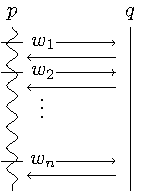
\includegraphics{./img/oracles/PPP.pdf}
            \caption{La macchina $M$ fa una computazione su $x$ limitata da $p(x)$ in tempo. In questa
            computazione fa, al piu', $p(x)$ interrogazioni all'oracolo su stringhe $w$ di lunghezza
        al piu' $p(x)$. La macchina $M'$ risponde alle interrogazioni di $M$ sostituendosi
    all'oracolo impiegando un tempo al piu' pari a $q(p(x))$.}
        \end{center}
    \end{figure}

    Quella che prima era un'interrogazione all'oracolo e che aveva costo $O(1)$ in $M$ ora ha, in
    $M''$, un costo polinomiale. Supponiamo che il polinomio che fa da bound a $M$ sia $p$ e il
    polinomio che fa da bound a $M'$ sia $q$. Le interrogazioni su stringhe di grandezza $n$
    all'oracolo costano, in $M''$, $q(n)$.
    
    Come calcoliamo la complessita' di $M''$? Dobbiamo calcolare quante saranno le interrogazioni
    all'oracolo. Queste sono sicuramente bound da $p(x)$. Ci chiediamo inoltre quanto possano essere
    grandi le stringhe $x$ che passiamo all'oracolo. Anche in questo caso la dimensione e' bound da
    $p(x)$. Di conseguenza abbiamo un bound alla complessita' di $M''$ uguale a
    $p(x)\cdot(q(p(x)))$. Ma questo e' un costo polinomiale. Di conseguenza esiste una MdT che
    riconosce $\Lang$ in tempo polinomiale, da cui $\PClass^{\PClass} \subseteq \PClass$.

    Abbiamo poi che, ovviamente, $\PClass \subseteq \PClass^{\PClass}$, da cui la tesi.
\end{proof}

Poniamo ora la nostra attenzione su $\PClass^{\NPClass}$. Se $\PClass \not= \NPClass$,
$\PClass^{\NPClass} \not= \PClass$. Abbiamo due ipotesi: o $\PClass^{\NPClass} = \NPClass$, oppure
e' qualcosa di ancora diverso (piu' grande di $\NPClass$).

\begin{figure}[h]
    \begin{center}
        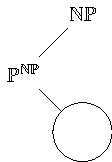
\includegraphics{./img/oracles/PNP.pdf}
        \caption{Allo stato attuale della conoscenza, $\PClass^{\NPClass}$ potrebbe coincidere con
        $\NPClass$ o essere qualcosa di totalemente diverso, piu' grande di $\NPClass$. Si
    congettura la seconda possibilita'.}
    \end{center}
\end{figure}

Supponiamo di avere quindi un oracolo per $\SAT$. Poiche' $\SAT$ e' $\NPClass$-completo possiamo
lavorare con un oracolo per $\SAT$ come se stessimo lavorando con un oracolo per un qualsiasi altro
linguaggio in $\NPClass$. Cosa riusciamo ora a calcolare? 

Ci chiediamo se possiamo rimpiazzare l'oracolo con una macchina deterministica. La macchina non
deterministica non rimpiazza bene l'oracolo, dato che esistono computazioni della MdTN che
falliscono. Un oracolo non deterministico risponde affermativamente in maniera corretta, ma potrebbe
rispondere negativamente perche' ha preso una computazione sfortunata. Di conseguenza dovremmo
rendere deterministica la macchina per rimpiazzare l'oracolo per $\SAT$. Ma usare una macchina
deterministica per simulare una macchina non deterministica ha un costo esponenziale, e cosi'
avremmo un costo esponenziale.

Potremmo immaginare di gestire la risposta dell'oracolo in maniera non deterministica, ma anche
questo ha le sue complicazioni.

Lavorando con un oracolo per $\SAT$ riusciamo a risolvere $\COSAT$ in tempo lineare, semplicemente
complementando la risposta. Ma sappiamo che $\COSAT \notin \NPClass$. Di conseguenza $\NPClass
\subseteq \PClass^{\NPClass}$ e $\CONPClass \subseteq \PClass^{\NPClass}$. Questo lascia presumere che
$\PClass^{\NPClass}$ sia diverso da $\NPClass$. Questo non e' stato dimostrato, ma lo si congettura.

Abbiamo invece che $\NPClass^{\PClass} = \NPClass$. Usare oracoli per $\PClass$ non ci aiuta se
usiamo macchine non deterministiche.

\section{Proprieta' delle classi con oracolo}

%Slide 146
Valgono le seguenti proprieta' per le classi di complessita' con oracolo:
\begin{thm}
    Per ogni linguaggio $A,B,C \in \Sigma^{*}$:
    \begin{itemize}
        \item $A \in \PClass^{A}$
        \item $A \in \PClass^{B} \implies A \in \NPClass^{B}$
        \item $A \in \NPClass^{B} \implies A \in \NPClass^{\Sigma^{*} \setminus B}$
        \item $A \in \PClass^{B} \land B \in \PClass^{C} \implies A \in \PClass^{C}$
        \item $A \in \NPClass^{B} \land B \in \PClass^{C} \implies A \in \NPClass^{C}$
    \end{itemize}
\end{thm}

Non e' detto che se $A \in \NPClass^{B}$ e $B \in \NPClass^{C}$, allora $A \in \NPClass^{C}$.

\begin{proof}
    La prima proprieta' e' ovvia. La seconda proprieta' e' una conseguenza del fatto che le macchine
    deterministiche sono un caso particolare di macchine non deterministiche. 

    Per gli oracoli si generalizzano molti teoremi gia' visti in teoria della complessita'. E' inoltre
    indentico lavorare con un oracolo per $B$ o per $\comp{B}$, dato che basta complementare la risposta
    per ottenere uno a partire dall'altro. 

    Il quarto punto e' una generalizzazione del teorema \ref{thm:PPP}. Il quinto punto ci dice che
    il fatto che il chiamante sia non deterministico si combina bene con il fatto che il chiamato
    sia deterministico. Viceversa quando il chiamato e' non deterministico abbiamo dei problemi
    nella composizione. Questo perche' la composizione con macchine non deterministiche e' piu'
    complessa. 

\end{proof}
%Slide 147

\begin{thm}
    Valgono le seguenti relazioni:
    \begin{enumerate}
        \item $\PClass^{\PClass} = \PClass$
        \item $\NPClass^{\PClass} = \NPClass$
        \item $\NPClass^{\PSPACE} = \PSPACE$
    \end{enumerate}
\end{thm}
\begin{proof}
    Andiamo per punti
        \begin{enumerate}
                \item Abbiamo gia' visto una dimostrazione di questo. Ne vediamo un'altra sfruttando
                    le proprieta' delle classi con oracolo. Abbiamo che $\PClass \subseteq
                    \PClass^{\PClass}$ poiche', per ogni linguaggio $A$, $A \in \PClass^{A}$.
                    Abbiamo poi che $\PClass^{\PClass} \subseteq \PClass$ poiche', per ogni
                    linguaggio $A,B,C$, $A \in \PClass^{B} \land B \in \PClass^{C} \implies A \in
                    \PClass^{C}$ e, in particolare, per $C = \emptyset$ otteniamo l'inclusione
                    voluta, da cui la tesi
                \item Analoga alla precedente
                \item $\PSPACE \subseteq \NPClass^{\PSPACE}$ poiche', per ogni linguaggio $A$, $A
                    \in \NPClass^{A}$. Per l'inclusione $\NPClass^{\PSPACE} \subseteq \PSPACE$,
                    supponiamo di avere una macchina non deterministica $M$ che lavora in tempo
                    polinomiale con un oracolo per un linguaggio $\Lang'$ in $\PSPACE$ e che
                    riconosce un linguaggio $\Lang \in \NPClass^{\PSPACE}$.  Possiamo immaginare di
                    sostituire all'oracolo una macchina deterministica $M'$ che lavora in spazio
                    polinomiale e riconosce $\Lang'$. Abbiamo un bound allo spazio usato da $M$,
                    dato dal polinomio $p$ che fa da bound al suo tempo.  Ci dobbiamo quindi
                    chiedere quale sia la dimensione delle stringhe di query.  Sappiamo, per il
                    teorema tempo-spazio, che queste possono avere al piu' dimensione polinomiale. 

                    Se quindi per riconoscere $\Lang'$ utilizziamo $M$ nelle parti di computazione
                    normale e utilizziamo $M'$ per simulare le interrogazioni all'oracolo, abbiamo
                    che lo spazio utilizzato e' dato da una composizione di polinomi. Di conseguenza
                    e' una computazione che puo' essere fatta in spazio polinomiale da una macchina
                    non deterministica, ovvero $\Lang \in \NPSPACE$. Dovremmo pero' passare ad una
                    macchina deterministica per concludere che $\Lang \in \PSPACE$. Ma sappiamo, per
                    il teorema di Savitch, che $\PSPACE = \NPSPACE$, poiche' una computazione non
                    deterministica che richiede spazio $p$ puo' essere simulata in modo
                    deterministico in $p^{2}$. Di conseguenza, $\Lang \in \PSPACE$.
        \end{enumerate}
\end{proof}

\begin{thm}\label{thm:oracles1}
    Abbiamo che $\NPClass \subseteq \PClass^{\NPClass} \subseteq \NPClass^{\NPClass}$.
\end{thm}
\begin{proof}
    $\NPClass \subseteq \PClass^{\NPClass}$, poiche' $\forall A. A \in \PClass^{A}$.
    $\PClass^{\NPClass} \subseteq \NPClass^{\NPClass}$, poiche' $\forall A,B. A \in \PClass^{B}
    \implies A \in \NPClass^{B}$.
\end{proof}

%Slide 153

\section{Gerarchia polinomiale}

La gerarchia polinomiale e' un analogo per la teoria della complessita' della gerarchia aritmetica
della teoria della calcolabilita. Anche in questo caso definiamo delle classi $\Sigma,\Pi,\Delta$.
Sono tutte classi di complessita' con complessita' polinomiale, che si suppone formino una
gerarchia.

Le classi base $\Sigma^{\PClass}_{0},\Pi^{\PClass}_{0}$ e $\Delta^{\PClass}_{0}$ sono coincidenti
con $\PClass$. Le classi $\Pi$ contengono i complementari dei linguaggi delle corrispettive classi
$\Sigma$. Nota: questo non significa che $\Pi_{n}^{\PClass} = \comp{\Sigma_{n}^{\PClass}}$, che e'
una cosa diversa.  Abbiamo che $\Pi_{n}^{\PClass} = \set{ \Lang \mid \comp{\Lang} \in
\Sigma_{n}^{\PClass}}$.

In particolare, definiamo:
\begin{itemize}
    \item $\Sigma_{n+1}^{\PClass} = \NPClass^{\Sigma_{n}^{\PClass}}$
    \item $\Pi_{n+1}^{\PClass} = \textbf{co-}\Sigma_{n+1}^{\PClass}$
    \item $\Delta_{n+1}^{\PClass} = \PClass^{\Sigma_{n}^{\PClass}}$
\end{itemize}

La classe $\PH$ e' la classe di tutti i linguaggi della gerarchia polinomiale:
\begin{equation*}
    \PH = \bigcup_{n \in \Nat}\Sigma_{n}^{\PClass}
\end{equation*}

Un fatto interessante e' che tutta la gerarchia polinomiale si sviluppa dentro un intervallo
abbastanza piccolo: e' tutta contenuta dentro $\PSPACE$. $\PH$ e' compresa tra $\PClass$ e
$\PSPACE$.

%Slide 154

Vediamo ora come sono organizzati i livelli della gerarchia

\begin{thm}
    Per ogni $n \in \Nat$ valgono le seguenti inclusioni:
    \begin{equation*}
        \Sigma_{n}^{\PClass} \cup \Pi_{n}^{\PClass} \subseteq \Delta_{n+1}^{\PClass} \subseteq
        \Sigma_{n+1}^{\PClass} \cap \Pi_{n+1}^{\PClass} \subseteq \PSPACE
    \end{equation*}
\end{thm}
\begin{proof}

    Sia $n \in \Nat$. Dimostriamo le inclusioni mostrando che $\Sigma_{n}^{\PClass} \subseteq
    \Delta_{n+1}^{\PClass}$, $\Pi_{n}^{\PClass} \subseteq \Delta_{n+1}^{\PClass}$,
    $\Delta_{n}^{\PClass} \subseteq \Sigma_{n+1}^{\PClass}$, $\Delta_{n}^{\PClass} \subseteq
    \Pi_{n+1}^{\PClass}$ e $\Sigma_{n}^{\PClass} \subseteq \PSPACE$:
    \begin{itemize}
        \item Abbiamo che, per ogni linguaggio $A$, $A \subseteq \PClass^{A}$; in particolare,
            questo vale per ogni linguaggio in
            $\Sigma_{n}^{\PClass}$. Di conseguenza, abbiamo che $\Sigma_{n}^{\PClass} \subseteq \PClass^{\Sigma_{n}^{\PClass}} =
            \Delta_{n+1}^{\PClass}$
        \item Abbiamo che, per ogni linguaggio $A$, lavorare con un oracolo per per $A$ o
            $\comp{A}$ e' equivalente. Ovvero, per ogni $A$, $A \subseteq \PClass^{\comp{A}}$.
            Poiche' $\Pi_{n}^{\PClass}$ contiene i complementari dei linguaggi in
            $\Sigma_{n}^{\PClass}$, abbiamo che $\Pi_{n}^{\PClass} \subseteq
            \PClass^{\Sigma_{n}^{\PClass}} = \Delta_{n+1}^{\PClass}$
        \item Abbiamo che per ogni linguaggio $A$, $\PClass^{A} \subseteq \NPClass^{A}$; in
            particolare, questo vale per i linguaggi in $\Sigma_{n}^{\PClass}$. Di conseguenza
            abbiamo che
            \begin{equation*}
                \Delta_{n+1}^{\PClass} = \PClass^{\Sigma_{n}^{\PClass}} \subseteq \NPClass^{\Sigma_{n}^{\PClass}} =
                \Sigma_{n+1}^{\PClass}
            \end{equation*}
        \item Abbiamo che le macchine deterministche sono chiuse per complementazione. Di
            conseguenza, per ogni linguaggio $A$, $\PClass^{A} = \COPClass^{A}$. In particolare,
            questo vale per i linguaggi in $\Sigma_{n}^{\PClass}$. Di conseguenza abbiamo che:
            \begin{equation*}
                \Delta_{n+1}^{\PClass} = \PClass^{\Sigma_{n}^{\PClass}} = \COPClass^{\Sigma_{n}^{\PClass}} \subseteq
                \CONPClass^{\Sigma_{n}^{\PClass}} = \Pi_{n+1}^{\PClass}
            \end{equation*}
        \item Dimostriamo per induzione su $n$ che $\Sigma_{n}^{\PClass} \subseteq \PSPACE$. Per $n = 0$
            abbiamo $\Sigma_{0}^{\PClass} = \PClass \subseteq \PSPACE$.

            Supponiamo ora che $\Sigma_{n}^{\PClass} \subseteq \PSPACE$. Abbiamo che $\Sigma_{n+1}^{\PClass} =
            \NPClass^{\Sigma_{n}^{\PClass}}$. Poiche' per ipotesi induttiva $\Sigma_{n}^{\PClass} \subseteq
            \PSPACE$, abbiamo che $\Sigma_{n+1}^{\PClass} \subseteq \NPClass^{\PSPACE}$. Ma
            $\NPClass^{\PSPACE} =
            \PSPACE$ per il teorema \ref{thm:oracles1}, da cui la tesi.
    \end{itemize}
\end{proof}

E' chiaro ora perche' la definizione di $\PH$ chiama in causa solo le classi $\Sigma$ e perche' e
sufficiente dimostrare che queste classi sono incluse in $\PSPACE$ per dimostrare che $\PH \subseteq
\PSPACE$: per ogni $n$, la classe $\Sigma_{n+1}^{\PClass}$ maggiora (contiene) le classi $\Delta_{n}^{\PClass}$
e $\Pi_{n}^{\PClass}$.

Si suppone che i vari livelli della gerarchia siano separati e che tutte le inclusioni che esistono
siano strette. Tuttavia cio' non e' stato dimostrato formalmente. Sappiamo che se $\PClass =
\NPClass$, allora la gerarchia polinomiale collasserebbe su $\PClass$. Allo stesso modo ci
potrebbero essere dei collassi parziali della gerachia: se $\NPClass=\CONPClass$ avremmo che la gerarchia
polinomiale collasserebbe su $\NPClass$. Questo si ritiene non essere vero, ma rimane una
possibilita' aperta al momento.

Possiamo vedere la gerarchia dal punto di vista delle classi $\Sigma,\Pi$ e $\Delta$ come illustrata
in figura \ref{img:PolyHierarchy1}. In termini di classi concrete, la gerarchia polinomiale e' come
illustrata in figura \ref{img:PolyHierarchy2}.

\begin{figure}[h]
    \begin{center}
        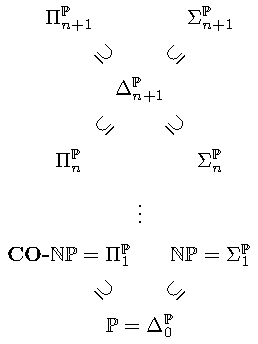
\includegraphics{./img/oracles/PolyHierarchy1.pdf}
        \caption{Rappresentazione della gerarchia polinomiale.}
        \label{img:PolyHierarchy1}
    \end{center}
\end{figure}

\begin{figure}[h]
    \begin{center}
        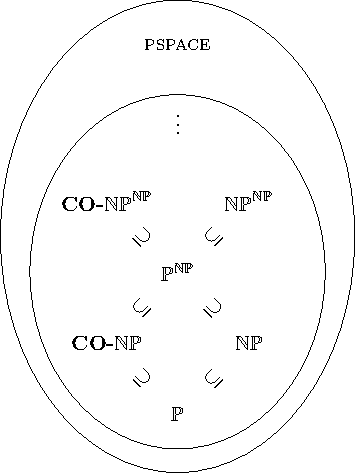
\includegraphics{./img/oracles/PolyHierarchy2.pdf}
        \caption{Rappresentazione della gerarchia polinomiale in funzione delle classi di
        complessita' concrete.}
        \label{img:PolyHierarchy2}
    \end{center}
\end{figure}

%Slide 156

Anche la gerarchia polinomiale puo' essere vista come una gerarchia definita da un alternarsi di
quantificazioni, cosi' come funzionava per la gerarchia aritmetica. Infatti, i problemi in
$\NPClass$ possono essere visti come proiezione esistenziale dei problemi in $\PClass$ con un bound
polinomiale alla dimensione del certificato. Il problemi in $\CONPClass$ sono proiezioni universali di
problemi in $\PClass$ con un bound polinomiale alla dimensione del certificato. Salendo nella
gerarchia abbiamo un discorso analogo: $\Sigma_{2}^{\PClass}$ contiene i problemi che sono
proiezione esitenziale di una proiezione universale di un problema in $\PClass$, e analogamente per
$\Pi_{2}^{\PClass}$. 

Il $\Sigma$ ci dice che il primo quantificatore nell'alternarsi di quantificatori della formula che
definisce la classe e' $\exists$ e $n$ ci dice quante volte dobbiamo alternare i quantificatori. Un
discorso analogo si applica a $\Pi$.
